\chapter{ANÁLISE DOS RESULTADOS DA  PESQUISA}
\label{chap:analise}

Esse Capítulo apresenta a análise dos dados obtidos em relação aos 2 (dois) instrumentos de coleta de dados (exercício de avaliação da DSL Cotas e o questionário aplicado com usuários), bem como, os resultados com os testes da API DSL Cotas. Esses instrumentos têm como foco verificar se a DSL Cotas atinge seus objetivos em relação à perspectiva dos usuários. 


Segundo \citeonline{poltronieri2018usability}, há muito esforço para criar e usar \gls{DSL}s como recurso de facilitar a construção do sistema, aumentar a produtividade e facilitar a manutenção. No entanto, as \gls{DSL}s tratam do problema de domínio (usuários especialistas) e não somente do domínio de solução (desenvolvedores/engenheiros de software), isso significa que nem sempre há aceitação e entendimento entre esses usuários.

Desse modo, os instrumentos de coleta descritos são utilizados de modo a identificar as dificuldades de uso entre diferentes tipos de usuários, por meio de aplicação prática da DSL e, posterior, aplicação de questionário. 

A fim de melhor sistematizar a organização dos dados optou-se por apresentar a análise por instrumento de coleta de dados e por grupo de usuários. Para tanto, a Subseção \ref{sec:analiseexercicio} expõe o resultados obtidos com o exercício prático proposto aos usuários convidados, assim como os resultados obtidos com a aplicação do questionário após a realização do exercício. As Subseções \ref{sec:avaliacaoapi} e \ref{sec:mudanasresultantes} detalham os resultados dos testes com a API e algumas mudanças aplicadas na DSL Cotas com base nas sugestões dos usuários.


Nesse sentido, considerando os diferentes perfis de usuário, os resultados foram agrupados de acordo com os 4 (quatro) grupos:  DEV-NESP; DEV-ESP; NDEV-ESP e NDEV-NESP, cujos perfis são definidos na Seção \ref{sec:idperfis}.


\section{Identificação dos perfis de usuários}
\label{sec:idperfis}


A Figura \ref{fig:perfilusuarios} apresenta o perfil de cada usuário que participou da avaliação de uso da DSL Cotas. Os critérios para inserção em cada grupo são descritos a seguir:

\begin{enumerate}
    \item[a)] \texttt{DEV-ESP}: usuários que possuem conhecimento sobre a lei Nº 12.711 e suas atualizações, são desenvolvedores e já atuaram em sistemas ou processos seletivos que utilizam o sistema de cotas;
    \item[b)] \texttt{DEV-NESP}: usuários com perfil de desenvolvedor sem conhecimento ou com conhecimento restrito sobre a legislação;
    \item[c)] \texttt{NDEV-ESP}: usuários com conhecimento na legislação, não desenvolvedores. Em sua maioria usuários que trabalham em setores que organizam processos seletivos relacionados ao sistema de cotas;
    \item[d)] \texttt{NDEV-NESP}: usuários não conhecedores da legislação e não desenvolvedores, de modo que pudesse ser identificado se as pessoas com esse perfil seriam capazes de aprender e de utilizar a DSL Cotas.
\end{enumerate}

\section{Informações obtidas com o questionário}
\label{sec:perguntasaplicadas}

Esta seção apresenta as perguntas do formulário \textit{on-line} submetido para todos os usuários participantes do presente estudo. As perguntas foram aplicadas após o término da execução do exercício, buscando obter as informações necessárias para cada perfil de usuário da DSL, assim como, entender as principais dificuldades encontradas por eles na utilização da linguagem.

As 5 (cinco) primeiras perguntas tem como objetivo levantar dados demográficos, tais como: nível de formação escolar, curso de formação acadêmica, cargo, tempo de experiência profissional e a informação se elas possuem experiência com desenvolvimento de sistemas.

Para levantar o conhecimento e experiência sobre sistema de cotas da rende de ensino federal foram submetidas as seguintes perguntas: "6. Você já atuou em sistemas ou processos seletivos que utilizam regras de classificação para candidatos cotistas?" e "7. Qual o seu grau de conhecimento sobre o sistema de cotas da Lei nº 12.711/2012 e suas atualizações?".

Em continuidade, foram adicionadas as seguintes perguntas responsáveis pelo levantamento de dificuldades de uso com a DSL:

\begin{enumerate}
    \item[a)] 8. Você já utilizou alguma Linguagem de Domínio Específica?;
    
    \item[b)] 9. De modo geral, qual o grau de dificuldade para execução do exercício proposto?;
    
    \item[c)] 10. Considerando a sua resposta na pergunta anterior, qual(is) a(s) dificuldade(s) encontrada(s)?;
    
    \item[d)] 11. Na sua avaliação quais as principais limitações da linguagem proposta?  ;
    
   \item[e)]  12. Quais dos materiais abaixo você utilizou para execução do exercício?;
   
   \item[f)] 13. No caso de a linguagem apresentar erros "destaques em vermelho" ou avisos "destaques em amarelo", as mensagens foram claras e ajudaram a resolver o(s) problema(s) apresentado(s)?;
   
   \item[g)] 14. Quanto tempo, aproximadamente, você utilizou para executar o exercício proposto?.   

\end{enumerate}

O formulário completo pode ser observado no (APÊNDICE \ref{chap:apen:formularioapen}). Os resultados obtidos com o formulário e os exercícios são descritos nas próximas Seções.


\begin{landscape}
\begin{figure}[ht!]
\centering

\caption{\textmd{Perfil dos usuários participantes}}
\label{fig:perfilusuarios}
\fcolorbox{gray}{white}{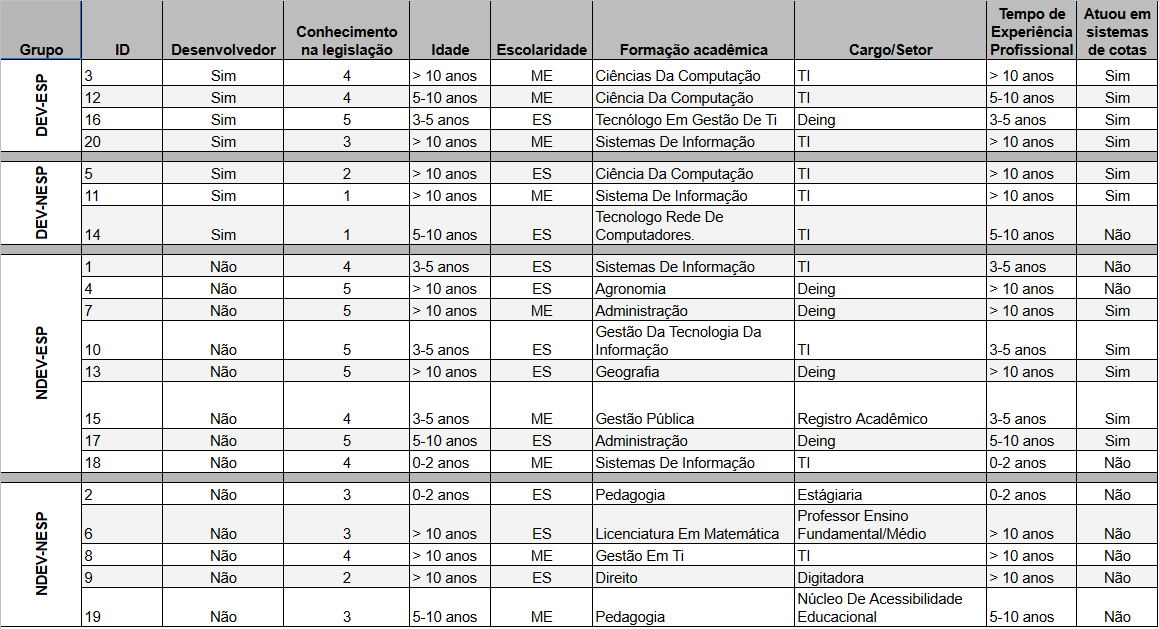
\includegraphics[width=1.5\textwidth]{chapters/analise/imagens/perfilusuarios.png}}

\par\medskip\textbf{Fonte:} Elaboração do autor (2020). \par\medskip

\end{figure}

\end{landscape}

\section{Resultados obtidos com o exercício}
\label{sec:analiseexercicio}

Cada usuário recebeu por e-mail um manual  contendo as principais instruções para uso da DSL Cotas, incluindo conceitos sobre cada elemento da legislação. Adicionalmente, a esse manual foi definido um exercício aberto, no qual, a tarefa proposta é definir os requisitos da primeira versão da lei nº 12.711 (Figura \ref{fig:exercicio}). 

\begin{figure}[ht!]
\centering

\caption{\textmd{Versão proposta para exercício da DSL}}
\label{fig:exercicio}
\fcolorbox{gray}{white}{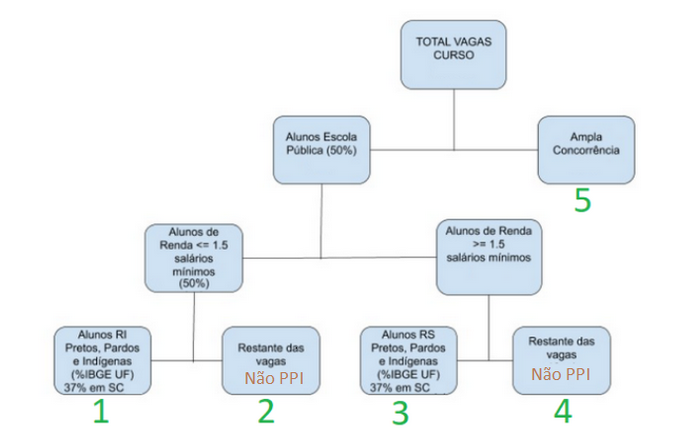
\includegraphics[width=0.85\textwidth]{chapters/analise/imagens/exercicio.png}}

\par\medskip\textbf{Fonte:} Elaboração do autor (2020). \par\medskip

\end{figure}



Essa versão foi escolhida por ser mais simples se comparada as versões mais recentes, requerendo um tempo menor de dedicação ao exercício e adequando a complexidade para todos os grupos dos diferentes perfis de usuários. 


Com o intuito de avaliar o exercício, todos os 20 exercícios foram salvos imediatamente após o término no sistema de controle de versão \texttt{git}. Cada usuário foi salvo em um \texttt{branch} disponível no repositório \texttt{https://github.com/spgroup/dsl-cotas/branches}.


Durante essa análise foram contabilizados os acertos em relação aos seguintes elementos da linguagem: distribuição de vagas (níveis e categorias criadas), configurações de percentuais (definição e utilização durante a distribuição), definição completa da ordem de prioridade (ordem indicada e quantidade de categorias presentes), quantidade de \textit{errors} e \textit{warnings} não resolvidos, e a presença de versão da legislação mais recente implementada opcionalmente por alguns usuários.

Desse modo, nas próximas Seções são apresentados os resultados da aplicação do exercício para cada grupo.

\newpage
\subsection{Resultados do Grupo DEV-ESP}
\label{subsec:devesp}

Em relação à pergunta "9. De modo geral, qual o grau de dificuldade para execução do exercício proposto?", em uma escala de 0(difícil) e 5(fácil), nesse grupo de usuários todos indicaram a nota 4 e 5. Ademais, foram realizadas as seguintes considerações:

 \begin{citacao}
 "Dúvidas de primeiro uso, do tipo -o que  mesmo que eu devia digitar maiúsculo?-, -será que preciso mesmo digitar 50.0 ou só 50?-,  entre outras do gênero. Como é execução de um exercício que é feito pela primeira vez, esse tipo de dúvida acaba não deixando totalmente fácil, pois eventualmente é necessário rever alguma instrução. Mas de resto, se já tiver esses detalhes na cabeça, a execução seria bem fácil (Usuário 20)."
\end{citacao}

Conforme relatado pelo Usuário 20, no primeiro contato com a DSL surgem algumas dúvidas sobre o formato de preenchimento dos percentuais e de siglas de categorias, o que pode levar a necessidade de reescrita de algumas instruções da linguagem. De modo geral isso pode ser resolvido a medida que se acostuma com a linguagem.

Outro aspecto levantado, relaciona-se com problemas durante a definição da ordem de prioridade, em que o comando de adição de novos itens na lista não estava claro o suficiente na linguagem, sendo necessário melhorar a usabilidade desse elemento:

\begin{citacao}
"A sequência de prioridades final onde se define quais candidatos se seleciona primeiro, foi um pouco mais difícil fazer a seleção... A dificuldade do último item pode ser melhorada com implementação ou instruções. No mais ficou bem interessante para configurar a árvore de decisão e percentuais aplicados (Usuário 3)." 
\end{citacao}

Os exercícios foram finalizados entre 15 a 30 minutos, sendo que 2 (dois) desses usuários (Usuário 20 e 16) fizeram completamente a definição da árvore de distribuição, sem \textit{errors} ou \textit{warnings}. Os outros dois usuários (Usuário 3 e 12) não resolveram alguns erros e avisos da linguagem, um deles criou um nível a mais de distribuição, gerando uma árvore de distribuição incorreta (Figura \ref{fig:errodevesp}). 

\begin{figure}[ht!]
\centering

\caption{\textmd{Exercício com erro na árvore de distribuição}}
\label{fig:errodevesp}
\fcolorbox{gray}{white}{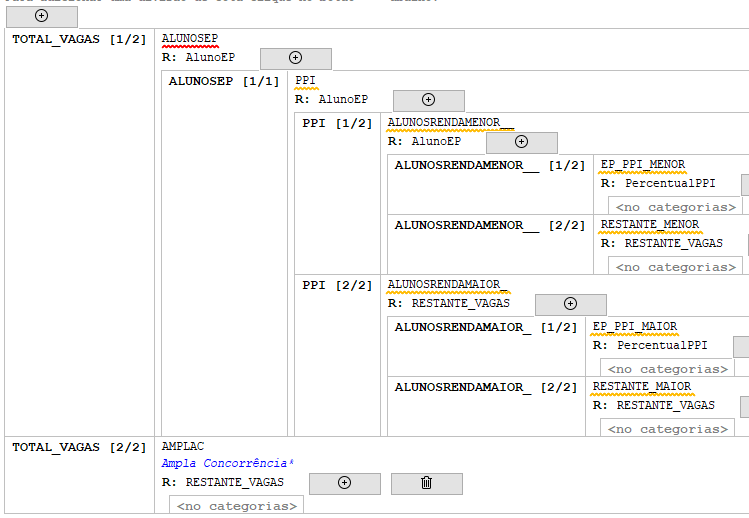
\includegraphics[width=0.85\textwidth]{chapters/analise/imagens/figerrodevesp.png}}

\par\medskip\textbf{Fonte:} Dados da pesquisa (2020). \par\medskip

\end{figure}



\newpage

\begin{figure}[ht!]
\centering

\caption{\textmd{Quadro da análise do grupo DEV-ESP}}
\label{fig:quadro:grupodevesp}
\fcolorbox{gray}{white}{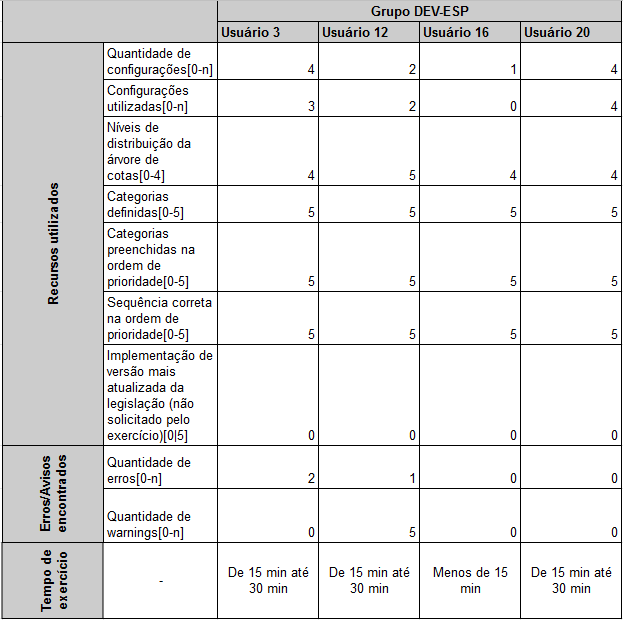
\includegraphics[width=0.85\textwidth]{chapters/analise/imagens/grupodevesp.png}}

\par\medskip\textbf{Fonte:} Elaboração do autor (2020). \par\medskip

\end{figure}



Com relação às assertivas presentes na questão "11. Na sua avaliação quais as principais limitações da linguagem proposta?", 2 (dois) usuários informaram que: "As sugestões das mensagens informativas não são claras o suficiente (Usuários 16 e 20)", o que pode ter levado aos problemas descritos anteriormente.

Em relação a pergunta "13. No caso de a linguagem apresentar erros "destaques em vermelho" ou avisos "destaques em amarelo", as mensagens foram claras e ajudaram a resolver o(s) problema(s) apresentado(s)?", esse grupo indicou conseguir de maneira geral resolver os problemas tendo como base as mensagens apresentadas pela DSL, todos indicaram a pontuação de escala 4 e 5 (quatro e cinco).

Contudo, após o levantamento apresentado na Figura \ref{fig:quadro:grupodevesp}, foi possível identificar que os demais recursos e percentuais foram preenchidos corretamente. Destaca-se que o grupo em análise, possui bom conhecimento na área de domínio, além de ter familiaridade com ferramentas de desenvolvimento e outras \gls{DSL}s, o que pode ter sido preponderante para que tenham indicado que a linguagem foi de fácil uso e entendimento. 

\newpage
\subsection{Resultados do Grupo DEV-NESP}
\label{subsec:devesp}

Neste grupo, com relação à pergunta sobre o grau de dificuldade, os usuários apontaram os níveis 3 e 2 (três e dois).  Conforme o levantamento descrito na Figura \ref{fig:quadro:grupodevnesp},  observou-se um tempo maior para o exercício do Usuário 5 (Mais de 30min), enquanto no exercício do Usuário 6 constaram vários erros não resolvidos na distribuição de vagas, em sua maioria em relação ao padrão de nomenclatura das siglas das categorias de cotas (Figura \ref{fig:errodevnesp}). 

\begin{figure}[ht!]
\centering

\caption{\textmd{Exercício do Usuário 11}}
\label{fig:errodevnesp}
\fcolorbox{gray}{white}{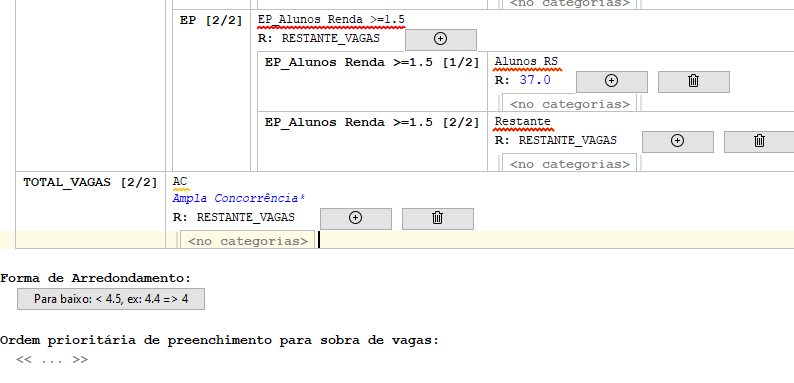
\includegraphics[width=0.85\textwidth]{chapters/analise/imagens/figerrodevnesp.png}}

\par\medskip\textbf{Fonte:} Elaboração do autor (2020). \par\medskip

\end{figure}



\begin{figure}[ht!]
\centering

\caption{\textmd{Quadro da análise do grupo DEV-NESP}}
\label{fig:quadro:grupodevnesp}
\fcolorbox{gray}{white}{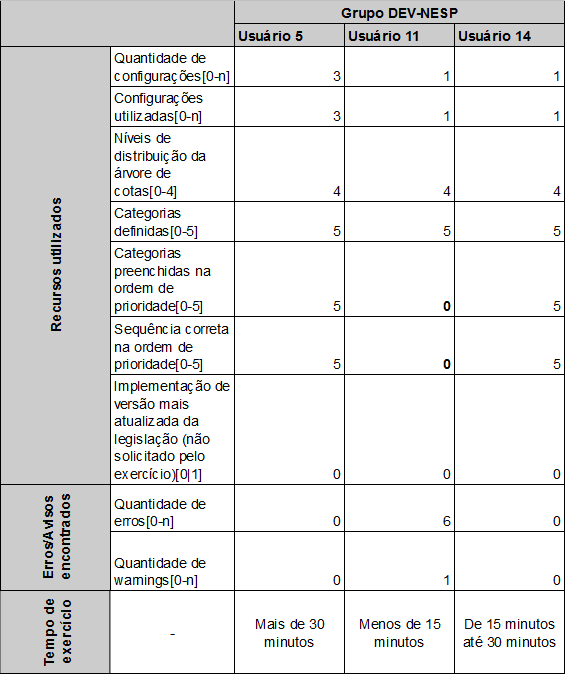
\includegraphics[width=0.77\textwidth]{chapters/analise/imagens/grupodevnesp.png}}

\par\medskip\textbf{Fonte:} Elaborada pelo autor (2020). \par\medskip

\end{figure}





Adicionalmente à questão sobre o grau de dificuldade foram feitos os seguintes comentários:

\begin{enumerate}
    \item [a)] "Foi difícil entender o funcionamento do sistema (Usuário 5)";
    \item [b)] "No exercício não compreendi se era pra utilizar a a ordem de prioridade ou não, se segue o padrão de uma árvore ou teria que informar. A questão do arredondamento ficou um pouco confusa, depois que entendi que é apenas uma configuração caso utilizar números quebrados nos percentuais (Usuário 11)";
    \item [c)] "Tive dificuldade em entender a proposta por não conhecer a lei especifica.  (Usuário 14)".    
\end{enumerate}

Portanto, nota-se a dificuldade de entendimento de questões relacionadas à legislação do sistema de cotas e adicionalmente algumas dificuldades sobre uso do elemento de ordem de prioridade da linguagem. 

Em continuidade a essa análise, apresentam-se as considerações sobre a questão assertiva sobre as limitações da linguagem: "Não observei a execução de uma emulação de processo em pratica (Usuário 5)", "As sugestões das mensagens informativas não são claras o suficiente (Usuário 11)".

Considerando a limitação apontada pelo Usuário 5, observa-se a falta do \textit{feedback} por parte da DSL para simulação em tempo real da distribuição de vagas, uma vez que a função responsável por fazer os cálculos do quadro de vagas foi implementada apenas na API DSL Cotas. 

Novamente foram apontados problemas nas mensagens geradas pela linguagem, conforme relato do Usuário 11. Esse usuário relata que: "O video didático poderia ser mais alto e com mais instruções de utilização.", indicando que são necessárias mais instruções, no manual e vídeo explicativo, pra conseguir melhorar o entendimento da linguagem. 

Ademais, as seguintes sugestões foram levantadas por meio da pergunta discursiva número 15 do questionário:

\begin{citacao}
A linguagem auxilia a documentar o processo. Acredito que ela implemente a execução da coleta de dados. Espero que ela saiba ler os dadas de varias bases diferentes, e não exija um tratamento nestes dados muito extenso, senão é talvez mais viável inserir diretamente os dados em uma base relacional e executar as ordenações necessárias (Usuário 5).
\end{citacao}

Tendo em vista os apontamentos descritos para o grupo, observa-se que a falta de entendimento nas regras de domínio dificulta o uso da linguagem (Usuários 11 e 14), no entanto há maiores preocupações relacionadas à simulação e à detalhes de implementação para o processamento final das regras (Usuário 5).

\newpage
\subsection{Resultados do Grupo NDEV-ESP}
\label{subsec:devesp}

\subsection{Resultados do Grupo NDEV-NESP}
\label{subsec:devesp}


\section{Resultados objetivos com a aplicação da API}
\label{sec:avaliacaoapi}


\section{Mudanças resultantes da avaliação}
\label{sec:mudanasresultantes}